\chapter{Annexes}
\section{Correction du CC1 Blanc}
\begin{exercice}~
    \begin{enumerate}
    \item $A = \dfrac{4^4 \cdot 3^3}{6^6 \cdot 2^2}$
    \begin{align*}
        A &= \frac{4^4 \cdot 3^3}{6^6 \cdot 2^2} \\
          &= \frac{(2^2)^4 \cdot 3^3}{(2 \cdot 3)^6 \cdot 2^2} \\
          &= \frac{2^8 \cdot 3^3}{2^6 \cdot 3^6 \cdot 2^2} \\
          &= 2^{8 - 6 - 2} \cdot 3^{3-6} \\
          &= 3^{-3} \\
          &= \frac{1}{3^3} \\
          \Aboxed{A &= \frac{1}{27}}
    \end{align*}
    \item $B = 6^{\frac{1}{2}} \cdot (\sqrt[5]{6})^3 \cdot - 2 \cdot 6^{\frac{1}{11}}$
    \begin{align*}
        B &= 6^{\frac{1}{2}} \cdot (\sqrt[5]{6})^3 \cdot - 2 \cdot 6^{\frac{1}{11}} \\
          &= 6^{\frac{1}{2}} \cdot (6^{\frac{1}{5}})^3 - 2 \cdot 6^{\frac{1}{11}} \\
          &= 6^{\frac{1}{2}} \cdot 6^{\frac{3}{5}} - 2 \cdot 6^{\frac{1}{11}} \\
        \Aboxed{B &= 6^{\frac{11}{10}} - 2 \cdot 6^{\frac{1}{11}} }
    \end{align*}
    \item $C = \dfrac{ 2\sqrt{2} 3\sqrt{3} \sqrt[3]{3} }{ 6 \sqrt[3]{6} \sqrt[6]{9} }$
    \begin{align*}
        C &= \dfrac{ 2\sqrt{2} 3\sqrt{3} \sqrt[3]{3} }{ 6 \sqrt[3]{6} \sqrt[6]{9} } \\
          &= \frac{2 \cdot 2^{\frac{1}{2}} \cdot  3 \cdot 3^{\frac{1}{2}} \cdot 3^{\frac{1}{3} }}{2 \cdot 3 \cdot 2^{\frac{1}{3}} \cdot 3^{\frac{1}{3}} \cdot (3^2)^{\frac{1}{6} } } \\
          &= \frac{ 2 \cdot 2^{ \frac{1}{2} } \cdot 3 \cdot 3^{ \frac{1}{2} } \cdot 3^{ \frac{1}{3} } }{ 2 \cdot 3 \cdot 2^{ \frac{1}{3} } \cdot 3^{ \frac{1}{3} } \cdot 3^{ \frac{1}{3} } } \\
          &= 2^{\frac{1}{6} - \frac{1}{3}} \cdot 3^{\frac{1}{2} - \frac{1}{3} } \\
        \Aboxed{C &= 6^{\frac{1}{6}}}
    \end{align*}
\end{enumerate}
\end{exercice}

\begin{exercice}~
    \begin{enumerate}
    \item Déterminer l'ensemble des réels $x$ qui vérifient :
    \begin{align*}
        (E) : &2x^2 + 6x + 4 \leq 0 \\ 
        \overset{\times \frac{1}{2}}{\iff} &x^2 + 3x + 2 \leq 0
    \end{align*}
    On cherche les racines du trinôme :
    \begin{align*}
        \Delta &= 3^2 - 4 \times 1 \times 2 \\
               &= 9 - 8 \\
               &= 1
    \end{align*}
    Les racines sont :
    \begin{align*}
        x_1 &= \frac{-3 - \sqrt{1}}{2} & x_2 &= \frac{-3 + \sqrt{1}}{2} \\
        \Aboxed{x_1 &= -2}             & \Aboxed{x_2 &= -1}                             
    \end{align*}
    On a donc le tableau de signes :
    \begin{figure}[h!]
        \centering
        \begin{tikzpicture}
            \tkzTabInit[lgt=2, espcl=2]
            {$x$ / 1,$x^2 + 3x + 2$ / 1}
            {$-\infty$, $-2$, $-1$, $+\infty$}
            \tkzTabLine{,+,z,-,z,+}
        \end{tikzpicture}
    \end{figure}
    \begin{figure}[h!]
        \centering
        \begin{align*}
            \Aboxed{(E) \iff x \in [-2, -1]}
        \end{align*}
    \end{figure}

    \item Déterminer l'ensemble des réels $x$ qui vérifient 
    \begin{align*}
        (E_1) : &x^2 + 5x + 7 \geq x + 5 \\
        \overset{-(x+5)}{\iff} &x^2 + 4x + 2 \geq 0
    \end{align*}
    On cherche les racines du trinôme :
    \begin{align*}
        &x^2 + 4x + 2 = 0 \\
        &\Delta = 4^2 - 4 \times 1 \times 2 = 8
    \end{align*}
    \begin{align*}
        x_1 &= \frac{-4 - \sqrt{8}}{2} & x_2 &= \frac{-4 + \sqrt{8}}{2} \\
            &= \frac{-4 - 2\sqrt{2}}{2} &    &= \frac{-4 + 2\sqrt{2}}{2} \\
        \Aboxed{x_1 &= -2 - \sqrt{2}} & \Aboxed{x_2 &= -2 + \sqrt{2}}
    \end{align*}
    On a le tableau de signes :
    \begin{figure}[h!]
        \centering
        \begin{tikzpicture}
            \tkzTabInit[lgt=2, espcl=2]
            {$x$ / 1, $x^2 + 4x + 2$ / 1}
            {$-\infty$, $-2 -\sqrt{2}$, $-2 + \sqrt{2}$, $+\infty$}
            \tkzTabLine{,+,z,-,z,+}
        \end{tikzpicture}
    \end{figure}
    \\
    On en conclut donc que :
    \begin{figure}[h!]
        \centering
        \begin{align*}
            \Aboxed{(E_1) \iff x \in ]-\infty, -2 - \sqrt{2}] \cup [-2 + \sqrt{2}, +\infty[}
        \end{align*}
    \end{figure}
\end{enumerate}
\end{exercice}

\begin{exercice}
    \par Déterminer l'ensemble des réels $x$ qui vérifient 
\begin{align*}
    (E) : |(x+1)(x+2)| = 10
\end{align*}
\par puis :
\begin{align*}
    (E') : |(x+1)(x+2)| \leq 10
\end{align*}
\par On sait que d'après la définition de la valeur absolue :
\begin{align*}
    (E) \iff
    \begin{cases}
        (E_1) : (x+1)(x+2) = 10 \\
        ou \\
        (E_2) : (x+1)(x+2) = -10
    \end{cases}
\end{align*}
\begin{align*}
    (E_1) : & (x+1)(x+2) = 10  & (E_2) : & (x+1)(x+2) = -10 \\
    \iff &x^2 + 3x + 2 = 10   & \iff &x^2 + 3x + 2 = -10 \\ 
    \iff &x^2 + 3x -8 = 0     & \iff &x^2 + 3x + 12 = 0 \\
    \Delta_1 &= 3^2 - 4 \times (-8) \times 1 & \Delta_2 &= 3^2 - 4 \times 12 \times 1 \\
    &= 41 & &= -39
\end{align*}
\par On remarque $(E_2)$ n'a pas de solution donc on cherche les racines de $(E_1)$.
\begin{align*}
    x_1 &= \frac{-3 - \sqrt{41}}{2} & x_2 &= \frac{-3 + \sqrt{41}}{2}
\end{align*}
\par L'ensemble des solutions de $(E)$ est : 
\fbox{$\{\frac{-3 - \sqrt{41}}{2}, \frac{-3 + \sqrt{41}}{2} \}$}

\begin{align*}
    |(x+1)(x+2)| = 
    \begin{cases}
        &(x+1)(x+2) \textnormal{ si } x \in ]-\infty;-2] \cup [-1;+\infty[ \\
        &-(x+1)(x+2) \textnormal{ si } x \in [-2;-1]
    \end{cases}
\end{align*}

\begin{itemize}
    \item $(x+1)(x+2) \leq 10$
    \begin{align*}
        &(x+1)(x+2) \leq 10 \\
        \iff &x^2 + 3x - 8 \leq 0\\
        \iff &x \in \left[\frac{-3 -\sqrt{41}}{2};\frac{-3 +\sqrt{41}}{2} \right]
    \end{align*}
    \par Sachant que $\dfrac{-3 -\sqrt{41}}{2} \leq \dfrac{-9}{2}$ car $-\sqrt{41} \leq 6$ et $\dfrac{-3+\sqrt{41}}{2} \geq 0$ car $\sqrt{41} \geq 6$ 
    \\
    \par Les solutions de $(x+1)(x+2) \leq 10$ dans $]-\infty,-2]\cup[1,+\infty[$ sont :
    \begin{align*}
        x \in \left[\dfrac{-3 - \sqrt{41}}{2},-2 \right]\cup \left[-1,\dfrac{-3 + \sqrt{41}}{2}\right]
    \end{align*}
    \item $-(x+1)(x+2) \leq 10$ 
    \begin{align*}
        &-(x+1)(x+2) \leq 10 \\
        \iff &x^2 + 3x + 12 \geq 0
    \end{align*}
    \par Ce qui est toujours vrai car ce trinôme n'a pas de racines.
    \par Ainsi, tout nombre de $[-2,-1]$ est solution de $-(x+1)(x+2) \leq 10$.
    \par Ainsi, l'ensemble des solutions de $(E')$ est :
    \begin{align*}
        &x \in \left[\frac{-3 - \sqrt{41}}{2}, -2\right] \cup \left[-1, \frac{-3 + \sqrt{41}}{2}\right]\cup \left[-2,-1\right] \\
        \Aboxed{&x \in \left[\frac{-3 - \sqrt{41}}{2}, \frac{-3 + \sqrt{41}}{2} \right]}
    \end{align*}
\end{itemize}
\end{exercice}

\begin{exercice}
    Déterminer l'ensemble des réels $x$ tels que les deux membres de (E) soient bien définis, et que (E) soit vraie
\begin{align*}
    (E) : \frac{1}{x-1} \leq \frac{x+4}{x+1}
\end{align*}
(E) est bien définie si $x \in \R \backslash \{-1,1\}$
\begin{align*}
    &\frac{1}{x-1} \leq \frac{x+4}{x+1} \\
    \iff &\frac{1}{x-1} - \frac{x+4}{x+1} \leq 0 \\
    \iff &\frac{(x+1) - (x+4)(x-1)}{(x-1)(x+1)} \leq 0 \\
    \overset{\times (-1)}{\iff} &\frac{(x+4)(x-1) - (x+1)}{(x-1)(x+1)} \geq 0 \\
    \iff &\frac{x^2 + 2x - 5}{(x+1)(x-1)} \geq 0
\end{align*}
On étudie le signe sachant qu'on a : 
\begin{itemize}
    \item $x+1 = 0 \iff x = -1$
    \item $x-1 = 0 \iff x = 1$
\end{itemize}
puis :
\begin{align*}
    &x^2 + 2x - 5 = 0 
\end{align*}
\begin{align*}
    \Delta &= 4 - 4 \times (-5) \times 1 \\
    &= 4 + 20 \\
    &= 24
\end{align*}
\begin{align*}
    x_1 &= \frac{-2 - \sqrt{24}}{2} & x_2 &= \frac{-2 + \sqrt{24}}{2} \\
        &= \frac{-2 - 2\sqrt{6}}{2} &     &= \frac{-2 + 2\sqrt{6}}{2} \\
    \Aboxed{x_1 &= -1 - \sqrt{6}} & \Aboxed{x_2 &= -1 + \sqrt{6}}
\end{align*}

\begin{figure}[h!]
    \centering
    \begin{tikzpicture}
        \tkzTabInit[lgt=2, espcl=2]
        {$x$/1, $(x+1)$ /1, $(x - 1)$ /1, $x^2 + 2x - 5$ /1, $\frac{x^2 + 2x - 5}{(x+1)(x-1)}$ /1}
        {$-\infty$, $-1 - \sqrt{6}$, $-1$, $1$, $-1 + \sqrt{6}$,$+\infty$}
        \tkzTabLine{,-,t,-,z,+,t,+,t,+}
        \tkzTabLine{,-,t,-,t,-,z,+,t,+}
        \tkzTabLine{,+,z,-,t,-,t,-,z,+}
        \tkzTabLine{,+,z,-,d,+,d,-,z,+}
    \end{tikzpicture}
\end{figure}
\clearpage
On en conclut que :
\begin{align*}
    \Aboxed{x \in ]-\infty, -1-\sqrt{6}]\ \cup \ ]-1,1[\ \cup \ [-1+\sqrt{6}, +\infty[}
\end{align*}
\end{exercice}

\begin{exercice}
    \par Une fonction $f:I \to J$ est surjective si et seulement si :
\begin{align*}
    \forall y \in J, \exists x \in I, f(x) = y
\end{align*}
\end{exercice}

\section{Correction CC Blanc 2}
\begin{exercice}~ 
\\
Rappel :
\begin{align*}
(u \circ v)' = v' \cdot u' \circ v 
\end{align*}
\begin{enumerate}
\item
$f(x) = \sin^3(x^2+1)$
Domaine de définition : $\R$
Pour calculer $f'$, on peut écrire 
\begin{align*}
f(x) = u \circ v(x) 
\begin{cases}
v(x) = x^2 +1 \\
u(x) = \sin^3(x)
\end{cases}
\begin{cases}
v'(x) = 2x \\
u'(x) = 3\cos(x)\sin^2(x)
\end{cases}
\end{align*}
d'où 
\begin{align*}
f'(x) &= 2x \cdot 3\cos(x)\sin^2(x) \\
	  &= 6x \cos(x) \sin^2(x)
\end{align*}

\item 
$g(x) = \ln(\tan(x))$
\\
$\tan$ est définie sur $\R \backslash \left\{ \frac{\pi}{2} + k\pi, k \in \Z \right\}$
\\
Pour $x \in \left[ -\frac{\pi}{2}, \frac{\pi}{2} \right]$
$\tan(x) > 0 \iff x \in \left[ 0, \frac{\pi}{2} \right]$
Comme $\tan$ est $\pi-$périodique, pour $x \in \left] k\pi - \frac{\pi}{2}, k \pi + \frac{\pi}{2} \right[ $
\\
$\tan(x) > 0 \iff x \in \left] k\pi, k\pi + \frac{\pi}{2} \right[$
\\
Domaine de définition : $\left] k \pi , k \pi + \frac{\pi}{2} \right[, k \in \Z$ 
\begin{align*}
\tan'(x) &= \frac{\sin'(x) \cos(x) - \sin(x) \cos'(x)}{\cos^2(x)} \\
         &= \frac{1}{\cos^2(x)}
\end{align*}
Par composition :
\begin{align*}
g'(x) &= \frac{\tan'(x)}{\tan(x)} \\
	  &= \frac{1}{\cos^2(x)\tan(x)} \\
	  &= \frac{1}{\cos(x)\sin(x)}
\end{align*}
\end{enumerate}
\end{exercice}

\begin{exercice}
    $u_0 = u_1 = 1$, $u_{n+1} = u_n + \frac{2}{n+1} u_{n-1}$
    \\
    Montrer que : $\forall n \in \N^*$, $u_n \leq n^2$\\
    Soit $P_n$ la propriété $"u_n \leq n^2$ \\
    Montrons $P_n$ par récurrence double.
    \\
    \textbf{Initialisation :}
    \\
    $u_1 = 1 \leq 1^2$ donc $P_1$ est vraie
    \\
    $u_2 = u_1 + \frac{2}{1+1} u_0 = 2 \leq 2²$ donc $P_2$ est vraie \\
    \textbf{Hérédité :}
    \\
    Pour $n \geq 2$, supposons que $P_{n-1}$ et $P_n$ vraies.
    \\
    Alors :
    \begin{align*}
        u_{n+1} &= u_n + \frac{2}{n+1} u_{n-1} \\
                &\leq n^2 + \frac{2}{n+1} (n-1)^2 \\
                &\leq n^2 + 2 (n - 1) \text{ car } \frac{n - 1}{n + 1} \leq 1 \\
                &\leq n^2 + 2n + 1 = (n + 1)^2
    \end{align*}
    Ainsi $P_{n+1}$ est vérifiée. Par récurrence double, on a montré $P_n$ pour tout $n \geq 1$
\end{exercice}

\begin{exercice}~
    \\
    $u_0 = 1$ \\
    $u_{n+1} = 1 + \frac{u_n}{2}$
    \begin{enumerate}
        \item On résout 
            \begin{align*}
                \alpha &= 1 + \frac{\alpha}{2} \\
                \iff \alpha &= 2
            \end{align*}
        et on étudie $v_n = u_n - 2$
        \begin{align*}
            v_{n+1} &= u_{n+1} - 2 \\
                    &= 1 + \frac{u_n}{2} - 2 \\
                    &= \frac{u_n}{2} - 1 \\
                    &= \frac{u_n - 2}{2} = \frac{v_n}{2}
        \end{align*}
        $v_0 = u_0 - 2 = - 1$
        La suite $(v_n)_{n \geq 0}$ est géométrique de premier terme $-1$ et de raison $\frac{1}{2}$, $\forall n \in \N$
        \begin{align*}
            v_n = -\frac{1}{2^n} \\
            u_n = 2 - \frac{1}{2^n}
        \end{align*}
    \item 
        Soit $n \in \N$
        \begin{align*}
            u_{n+1} - u_n &= \left( 2 - \frac{1}{2^{n+1}} \right) - \left( 2 - \frac{1}{2^n} \right) \\
                          &= \frac{1}{2^n} - \frac{1}{2^{n+1}} \\
                          &= \frac{2}{2^{n+1}} - \frac{1}{2^{n+1}} \\
                          &= \frac{1}{2^{n+1}} \geq 0
        \end{align*}
        \item 
            Comme $\frac{1}{2^n} \xrightarrow[n \to +\infty]{} 0$, la suite $(v_n)_{n \geq 0}$ converge vers 2.
    \end{enumerate}
\end{exercice}

\begin{exercice}
$n > 0$, $u_n \frac{\sin}{\sqrt{n}} + \frac{n+1}{n+2}$
\begin{align*}
    \frac{n+1}{n+2} &= \frac{n + 2 - 1}{n + 2} = 1 - \frac{1}{n+2} \\
                    &\text{ OU } \\
    \frac{n+1}{n+2} &= \frac{n\left( 1 + \frac{1}{n}\right)}{n\left( 1 + \frac{2}{n} \right)} = \frac{1 + \frac{1}{n}}{1 + \frac{2}{n}}
\end{align*}
Sachant que 
\begin{align*}
\lim_{n \to +\infty} \frac{1}{n+2} = \lim_{n \to +\infty} \frac{1}{n} = \lim_{n \to +\infty} \frac{2}{n} =  0
\end{align*}
On a :
\begin{align*}
    \lim_{n \to +\infty} \frac{n+1}{n+2} = 1
\end{align*}

$\forall n \in \N$
\begin{align*}
    -\frac{1}{\sqrt{n}} \leq \frac{\sin(x)}{\sqrt{n}} \leq \frac{1}{\sqrt{n}}, \text{ car } -1 \leq \sin (x) \leq 1
\end{align*}
\begin{align*}
    \lim_{n \to +\infty} -\frac{1}{\sqrt{n}} = \lim_{n \to +\infty} \frac{1}{\sqrt{n}} = 0
\end{align*}
Par le théorème  des gendarmes 
\begin{align*}
    \lim_{n \to +\infty} \frac{\sin(x)}{\sqrt{n}} = 0
\end{align*}
Finalement 
\begin{align*}
    u_n \xrightarrow[n \to +\infty]{} 1
\end{align*}
\end{exercice}

\begin{exercice}
    Résoudre 
    \begin{align}\label{exercice5_correction_equation}
        \sqrt{3} \sin(3x) - \cos(3x) = \sqrt{2}
    \end{align}
Méthode : se ramener à une équation de type $\sin(\cdots) = \sin(\cdots)$ ou $\cos(\cdots) = \cos(\cdots)$ à l'aide des formules d'addition.
    \begin{align*}
        (\ref{exercice5_correction_equation}) &\iff \frac{\sqrt{3}}{2} \sin(3x) - \frac{1}{2} \cos(3x) = \frac{\sqrt{2}}{2} \\
                                         &\iff \cos\left(\frac{\pi}{6}\right)\sin(3x) - \sin\left(\frac{\pi}{6}\right)\cos(3x) = \frac{\sqrt{2}}{2} \\
                                         &\iff \sin\left(3x - \frac{\pi}{6}\right) = \sin\left(\frac{\pi}{4}\right)
    \end{align*}
    \begin{align*}
        \sin(a) = \sin(b) \iff 
        \begin{cases}
            a = b + 2k\pi, (k \in \Z) \\
            a = \pi - b +2k\pi, (k \in \Z)
        \end{cases}
    \end{align*}
    \begin{align*}
        (\ref{exercice5_correction_equation}) &\iff 
        \begin{cases}
            3x - \frac{\pi}{6} = \frac{\pi}{4} + 2k\pi, (k \in \Z) \\
            \text{ou} \\
            3x - \frac{\pi}{6} = \pi - \frac{\pi}{4} + 2k \pi, (k \in \Z) 
        \end{cases}
                                         &\iff
        \begin{cases}
            3x = \frac{5\pi}{12} + 2k\pi, (k \in \Z) \\
            \text{ou} \\
            3x = \frac{11\pi}{12} + 2k\pi, (k \in \Z)
        \end{cases}
    \end{align*}
	\begin{align*}
		\begin{cases}
			x = \frac{5\pi}{36}+ \frac{2k\pi}{3}, (k \in \Z) \\
			\text{ou} \\
			x = \frac{11\pi}{36} + \frac{2k\pi}{3}, (k \in \Z)
		\end{cases}
	\end{align*}
\end{exercice}